% vim:set et fenc=utf-8 ft=tex sw=2 ts=2 tw=72:

\newif\ifdraft
%\drafttrue

\ifdraft
        \documentclass[draft]{IEEEtran}
        \def\baselinestretch{1}
        % \setlength{\marginparwidth}{1.5cm}
\else
        \documentclass[conference]{IEEEtran}
\fi

\usepackage[T1]{fontenc}
\usepackage[utf8]{inputenc}
\usepackage[hyphens]{url}
\urlstyle{same}

%% Citations
\usepackage[nospace]{cite}

%% Table Support
\usepackage{array}
\usepackage{dcolumn}
\usepackage{longtable}
\usepackage{multirow}
\usepackage{booktabs}
\usepackage{tabulary}

%% Extra support
\usepackage{xspace}
\usepackage{amsmath}
\usepackage{balance}
\usepackage{placeins}

%% Algorithms
\usepackage{algorithm}
\usepackage{algpseudocode}

%% Graphics
\usepackage{tikz}
\usepackage{pgfplots}
\usepackage{pgfplotstable}
\usepackage{xcolor}
\usepackage{color}
\usepackage{listings}


\usetikzlibrary{positioning, arrows}

\input{color.tex}
% \ifdraft
%     \usepackage[colorinlistoftodos]{todonotes}
%     \newcommand{\evan}[1]{{\color{blue}\emph{Evan Says: #1}}\xspace}
%     \newcommand{\evantodo}[1]{{\color{blue}\emph{Evan Todo: #1}}\xspace}
%     \newcommand{\dmg}[1]{{\color{blue}\emph{dmg Says: #1}}\xspace}
%     \newcommand{\dmgtodo}[1]{{\color{blue}\emph{dmg Todo: #1}}\xspace}
% \else
%     \usepackage[disable]{todonotes}
%     \newcommand{\evan}[1]{}
%     \newcommand{\evantodo}[1]{}
%     \newcommand{\dmg}[1]{}
%     \newcommand{\dmgtodo}[1]{}
% \fi

\newcommand{\tool}{{\emph Linvis}\xspace}

\ifdraft
    \usepackage[colorinlistoftodos]{todonotes}
    \newcommand{\evan}[1]{{\color{blue}\emph{Evan Says: #1}}\xspace}
    \newcommand{\evantodo}[1]{{\color{blue}\emph{Evan Todo: #1}}\xspace}
    \newcommand{\dmg}[1]{{\color{blue}\emph{dmg Says: #1}}\xspace}
    \newcommand{\dmgtodo}[1]{{\color{blue}\emph{dmg Todo: #1}}\xspace}
\else
    \usepackage[disable]{todonotes}
    \newcommand{\evan}[1]{}
    \newcommand{\evantodo}[1]{}
    \newcommand{\dmg}[1]{}
    \newcommand{\dmgtodo}[1]{}
\fi

\newcommand{\mycode}[1]{\texttt{\small #1\xspace}}


%%% Local Variables:
%%% mode: plain-tex
%%% TeX-master: t
%%% End:


\newcommand{\TheTitle}{Merge-Tree: Visualizing the Integration of Commits into Linux}
\newcommand{\TheAuthors}{Evan Wilde, Daniel M. German}
\newcommand{\TheEmails}{etcwilde@uvic.ca, dmg@uvic.ca}
\newcommand{\TheSubject}{Understanding a large number of commits and merges}
\newcommand{\TheKeywords}{Linux, git, visualizations}

%% Referencing
\usepackage[unicode=true,
          pdftitle={\TheTitle},
          pdfauthor={\TheAuthors},
          colorlinks=false]{hyperref}


\algdef{SE}[DOWHILE]{Do}{doWhile}{\algorithmicdo}[1]{\algorithmicwhile\ #1}%

\lstset{frame=tb,
  language=python,
  aboveskip=3mm,
  belowskip=3mm,
  showstringspaces=false,
  columns=flexible,
  basicstyle={\small\ttfamily},
  numbers=none,
  numberstyle=\tiny\color{gray},
  keywordstyle=\color{chartblue},
  commentstyle=\color{chartred},
  stringstyle=\color{chartgreen},
  breaklines=true,
  breakatwhitespace=true,
  tabsize=3
}

\synctex=1

\begin{document}

\title{\TheTitle}

\author{
        \IEEEauthorblockA{\TheAuthors}
        \IEEEauthorblockN{Department of Computer Science,
                University of Victoria, Canada.}
        \IEEEauthorblockA{Email: \TheEmails}
}
\maketitle

\begin{abstract}

  With an average of more than 900 top-level merges into the Linux
  kernel per release, many containing hundreds of commits and some
  containing thousands, maintenance of older versions of the kernel
  becomes nearly impossible.  Various commercial products, such as the
  Android platform, run older versions of the kernel. Due to security,
  performance, and changing hardware needs, maintainers must understand
  what changes (commits) are added to the current version of the kernel
  since the last time they inspected it in order to make the necessary
  patches.

  Current tools provide information about repositories through the
  directed acyclic graph (DAG) of the repository, which is helpful for
  smaller projects. However, with the scale and number of branches in
  the kernel the DAG becomes overwhelming very quickly. Furthermore, the
  DAG contains every ancestor of every commit, while maintainers are
  more interested in how and when a commit arrives to the official Linux
  repository.

  In this paper, we propose the merge-tree, a simplified transformation
  of the DAG of the Linux git repository that shows the way in which
  commits are merged into the master branch of Linux. Using the
  merge-tree, we build \tool, a tool that is designed to allow users to
  explore how commits are merged into the Linux kernel.

\end{abstract}


\begin{IEEEkeywords}
  \TheKeywords
\end{IEEEkeywords}

\section{Introduction}

Between 50k and 70k commits are added to the Linux kernel per version
requiring maintainers of older versions of the kernel to sift through
thousands of commits and merges with tools that are unable to filter and
effectively visualize projects at the scale of the kernel. Older
versions of the kernel are used in embedded systems and mobile phones;
for security purposes, performance needs, and changing hardware
requirements, maintainers must be able to understand the changes being
made in the current version of the kernel in order to produce the
necessary patches for the older versions of the kernel. Tools like Gitk
use a directed acyclic graph (DAG) model of the repository, showing all
commits and merges in chronological order by when the commit was
authored, not by when it arrived in the official Linux repository.

\begin{figure*}
        \centering
        \includegraphics[width=0.97\textwidth]{figures/gitk.png}
        \caption{A view of the Gitk interface centered on merge
          b34870fc9ff15fe46c4066faeeec437a4e63e2d8 by Miller. Commits point toward
          their ancestors and there is no clear path from the commit to the merge
          with the master branch. Neither Gitk nor Git are capable of showing the
          commits in master.}
        \label{fig:gitk}
%\vspace{-4mm}
\end{figure*}


\begin{figure}
        \centering
        \includegraphics[width=0.45\textwidth]{figures/github_viewer.png}
        \caption{Github Failure Message showing the DAG of the Linux Project and its
                relationship to other forks.}
        \label{fig:gitfail}
%\vspace{-2mm}
\end{figure}


This representation works in smaller projects; it enables users to see
when changes are made, when these changes are merged, how each branch is
interacting, and the point where a branch forks from the master branch.
In large modular projects, like the Linux kernel, the DAG becomes a mess
of merges and commits (Figure~\ref{fig:gitk}) losing its visual meaning.
In some cases, the Linux kernel is simply too large for the system to
generate a visualization; Github provides a DAG view for many projects,
but is unable to display the visualization for projects at the scale of
the Linux of the kernel (Figure~\ref{fig:gitfail}).  Between 60k and 70k
new commits are created for the Linux project every year; according to
our previous work\cite{German2015}, a commit takes a median of 30 days
from the time it is authored until it arrives in the official
repository. The snapshot of the kernel tomorrow may be different than
the snapshot from today, containing new commits authored in the past;
distinguishing these new commits from the commits in the snapshot from
today is not trivial.


One major challenge with visualizing the arrival of commits to a
repository is that Git does not store the date that a commit was merged
into another branch, including the master branch. To complicate the
problem, the DAG only has references to the ancestors of a commit (a
model necessary for the operation of Git), but maintainers would prefer
knowing the path a commit followed to reach the master repository.
Tracing a path that any commit followed to the master repository would
imply that for any given merge, it would be possible to know which
commits were merged. A user could inspect the commits that arrived into
the master branch within a given time-frame by checking which commits
were merged during that time-frame.

This paper makes two contributions; first, we describe a method of
converting the DAG of the Linux repository into a tree, or
\emph{merge-tree} of the repository, that represents the path used by a
commit to reach the master branch; second, we present a method to
inspect and visualize the history of merges in the Linux project using
the merge-tree model.

These methods and visualizations are implemented in a web-based tool
called \tool\footnote{\tool is currently available at
  \url{http://li.turingmachine.org}}.  Our visualizations and tool
provide information about the location of any given commit or merge in
its respective merge-tree, the files edited, the modules edited, and the
commit message. \tool allows users to apply various filters, including
the release version, along with a keyword or phrase from the log
preview, the name of the author, or the commit ID. The user can request
all merges made by Linus that contain a commit or inner merge that
matches the search query, or just the commits and merges that match the
query.

\section{Merge-Tree model}
\label{sec:mergetree}

Git uses a directed acyclic graph (DAG) as its main data model. In this
model, a commit has one or more ordered parents (ancestors), except the
root commits of a repository which do not have ancestors--Linux's git
repository has two such commits.  Commits are divided into merge
commits, merging two or more branches, and non-merge commits. Non-merge
commits have only one parent, while merge commits have two or more. The
order of the parents matter: the first parent is the branch in which the
merge is being done, while the rest indicate the branches being merged
(Git allows merging multiple branches simultaneously). The second parent
is the first branch merged, the third parent is the second branched
merged, etc.

Once a commit is created, it is never changed. Git allows operations to
alter commits or reorder them, but it changes the commit ID in the
process, effectively replacing it with a new commit. This makes commits
unable to record the traversal of merges from the commit to the merge
into the master branch.

A short example: assume the commits represented in
Figure~\ref{fig:repoEvents} show the sequence of events in a repository.
In this case, commits are performed in various repositories and
branches. The DAG representation of the commits is shown in
Figure~\ref{fig:repoDAG}. Notice that the DAG loses information about
the master branch and the repository that the master branch is part of.
The merge-tree view of this DAG is visible in Figure~\ref{fig:repoTree}.
Note that the direction of the edges of the DAG have been inverted,
instead of pointing from the child to the ancestors, it points from the
ancestor to its successors, forming a path to the master branch. Also
note that the DAG has been simplified, showing only a single edge on the
path to master for any commit.

\begin{figure}[htbp]
  \centering
  \begin{tikzpicture}[auto, on grid, semithick, state/.style={circle, text=black}]
    \foreach \x in {0, 1, 2, 3, 4, 5, 6, 7}
    \draw[shift={(\x + 0.5, -0.5)}, color=black] (0cm, 4cm) -- (0pt, -0.2cm);

    \node[state, draw=chartblue] (1) {1};
    \node[state, draw=chartyellow, above right= of 1] (2) {2};
    \node[state, draw=chartmagenta, above right= 2cm and 1cm of 2] (3) {3};
    \node[state, draw=chartblue, right= 2cm of 1] (4) {4};
    \node[state, draw=chartyellow, above right=of 4] (5) {5};
    \node[state, draw=chartred, above right=of 5] (6) {6};
    \node[state, draw=chartyellow, right=of 5] (7) {7};
    \node[state, draw=chartmagenta, above right= 2cm and 1cm of 7](8) {8};
    \node[state, draw=chartyellow, right= 2cm of 7] (9) {9};
    \node[state, draw=chartyellow, right=of 9] (10) {10};
    \node[state, draw=chartblue, below right=of 9] (11) {11};
    \node[state, draw=chartblue, below right=of 10] (12) {12};

    \draw (12) edge[-stealth] (11) edge[chartyellow, -stealth] (10);
    \draw (11) edge[-stealth] (4) edge[chartyellow, -stealth] (9);
    \draw (10) edge[chartyellow, -stealth] (9);
    \draw (9) edge[chartmagenta, -stealth] (8) edge[chartred, -stealth] (6)
              edge[chartyellow, -stealth] (7);
    \draw (8) edge[chartmagenta, -stealth] (7);
    \draw (7) edge[chartyellow, -stealth] (5);
    \draw (6) edge[chartred, -stealth] (5);
    \draw (5) edge[chartmagenta, -stealth] (3) edge[chartyellow,-stealth] (2)
              edge[chartyellow, -stealth] (4);
    \draw (4) edge[-stealth] (1);
    \draw (3) edge[chartmagenta, -stealth] (2);
    \draw (2) edge[chartyellow, -stealth] (1);

    \node [draw=chartblue, below = 1.5cm of 1] (l1) {Master};
    \node [draw=chartyellow, right = 1.5cm of l1] (l2) {Repo A};
    \node [draw=chartred, right = 2.5cm of l2] (l3) {Branch of Repo A};
    \node [draw=chartmagenta, right= 2.5cm of l3] (l4) {Repo B};

        \foreach \x in {0, 1, 2, 3, 4, 5, 6, 7, 8}
    \node[shift={(\x, -0.6)}, color=black] {$t_\x$};
  \end{tikzpicture}
  \caption{Example of a sequence of events performed in different
    repositories. The horizontal axis represents time. Each horizontal
    section represents a different branch and/or repository. Each commit
    points to its ancestor.}
  \label{fig:repoEvents}
%\vspace{-3mm}
\end{figure}

\begin{figure}[htbp]
  \centering
  \begin{tikzpicture}[auto, on grid, semithick, state/.style={circle, text=black}]
    \node[state, draw=chartblue] (1) {1};
    \node[state, draw=chartyellow, above right= of 1] (2) {2};
    \node[state, draw=chartmagenta, above right= 2cm and 1cm of 2] (3) {3};
    \node[state, draw=chartblue, right= 2cm of 1] (4) {4};
    \node[state, draw=chartyellow, above right=of 4] (5) {5};
    \node[state, draw=chartred, above right=of 5] (6) {6};
    \node[state, draw=chartyellow, right=of 5] (7) {7};
    \node[state, draw=chartmagenta, above right= 2cm and 1cm of 7](8) {8};
    \node[state, draw=chartyellow, right= 2cm of 7] (9) {9};
    \node[state, draw=chartyellow, right=of 9] (10) {10};
    \node[state, draw=chartblue, below right=of 9] (11) {11};
    \node[state, draw=chartblue, below right=of 10] (12) {12};

    \draw (12) edge[-stealth] (11) edge[chartyellow, -stealth] (10);
    \draw (11) edge[-stealth] (4) edge[chartyellow, -stealth] (9);
    \draw (10) edge[chartyellow, -stealth] (9);
    \draw (9) edge[chartmagenta, -stealth] (8) edge[chartred, -stealth] (6)
              edge[chartyellow, -stealth] (7);
    \draw (8) edge[chartmagenta, -stealth] (7);
    \draw (7) edge[chartyellow, -stealth] (5);
    \draw (6) edge[chartred, -stealth] (5);
    \draw (5) edge[chartmagenta, -stealth] (3) edge[chartyellow,-stealth] (2)
              edge[chartyellow, -stealth] (4);
    \draw (4) edge[-stealth] (1);
    \draw (3) edge[chartmagenta, -stealth] (2);
    \draw (2) edge[chartyellow, -stealth] (1);
  \end{tikzpicture}
  \caption{DAG representation of the commits represented in
    Figure~\ref{fig:repoEvents}. The DAG loses information about which
    repository the commit is performed in and through which merges it
    has passed on its way to the master branch. The DAG does not even
    distinguish the master branch from other branches.}
  \label{fig:repoDAG}
%\vspace{-3mm}
\end{figure}

\begin{figure}[htbp]
  \centering
  \begin{tikzpicture}[auto, on grid, semithick, state/.style={circle, text=black}]

    \draw[chartblue]
      (-0.5, -0.5) -- (8.5, -0.5) -- (8.5, 0.5) -- (-0.5, 0.5) -- (-0.5, -0.5);

    \node[state, draw=chartblue] (1) {1};
    \node[state, draw=chartyellow, above right= of 1] (2) {2};
    \node[state, draw=chartmagenta, above right= 2cm and 1cm of 2] (3) {3};
    \node[state, draw=chartblue, right= 2cm of 1] (4) {4};
    \node[state, draw=chartyellow, above right=of 4] (5) {5};
    \node[state, draw=chartred, above right=of 5] (6) {6};
    \node[state, draw=chartyellow, right=of 5] (7) {7};
    \node[state, draw=chartmagenta, above right= 2cm and 1cm of 7](8) {8};
    \node[state, draw=chartyellow, right= 2cm of 7] (9) {9};
    \node[state, draw=chartyellow, right=of 9] (10) {10};
    \node[state, draw=chartblue, below right=of 9] (11) {11};
    \node[state, draw=chartblue, below right=of 10] (12) {12};

    \draw (2) edge[chartyellow, -stealth] (5)
          (3) edge[chartmagenta, -stealth](5)
          (5) edge[chartyellow, -stealth] (7)
          (7) edge[chartyellow, -stealth] (9)
          (6) edge[chartred, -stealth] (9)
          (8) edge[chartmagenta, -stealth] (9)
          (9) edge[chartyellow, -stealth] (11)
          (10) edge[chartyellow, -stealth] (12);


  \end{tikzpicture}
  \caption{Merge-tree view of the commits  represented in
    Figure~\ref{fig:repoEvents} showing the path they followed to reach
    the master branch. In this model the successors of each commit
    represents the path followed by that commit to reach the master
    branch.}
  \label{fig:repoTree}
\vspace{-3mm}
\end{figure}

\subsection{Computing the merge-tree of the DAG of Linux}

Computing the merge-tree from a DAG for any repository may not be
possible; however, certain features of the development process of Linux
make it feasible to compute the merge-tree for the Linux repository.
First, the master branch of Linux is maintained by Linus Torvalds, and
only Linus has write access to it. We have verified this assertion in
previous research~\cite{German2015}. We have developed a heuristic that
is presented in Algorithm~\ref{fig:alg}. In short, the algorithm first
identifies the commits made directly to the master branch; whereafter it
recursively determines the shortest path (in terms of time), using the
DAG, from each commit to the master branch using the inverted DAG.

\begin{algorithm}
        \caption{Computing the merge-tree of Linux Git's DAG}\label{fig:alg}
        \begin{algorithmic}
                \Function{ComputeMergeTree}{DAG}: tree
                \State {\# Compute the tree from the DAG of Linux repository.}
                \State {\# Returns $Tree$, a graph containing every commit }
                \State {\# in DAG with the path it followed to master.}

                \State $head \gets \textit{Head of master of git repository}$
                \State $master \gets \textit{traverse DAG from head using }$
                \State \quad\quad\quad\quad $\textit{first ancestor until reaching root}$
                \State $nodes(Tree) \gets nodes(DAG)$
                \State \Function{distance2Master}{cid} : seconds
                \State {\# Helper function}
                \State {\# Recursively compute shortest distance to master}
                \State {\# setting cid's successor (next) in its way to master.}
                \State {\# This function should be memoized. Otherwise it}
                \State {\# would run in exponential time.}
                \If {\textit{cid in master}}
                \State \Return 0
                \EndIf
                \State    $d \gets 	\infty$
                \State {\# Traverse the inverted DAG}
                \For{$c \in children(cid, DAG)$}
                \If {$c \in master$}
                \State $d_1 \gets commitTime(c)-commitTime(cid)$
                \Else
                \State {$d_1 \gets distance2Master(c)$}
                \EndIf
                \If {$d_1 < d $}
                \State $next \gets c$
                \State  $d \gets d_1$
                \EndIf
                \EndFor
                \State {\# $c$ is the commit that follows $cid$}
                \State {\# in its way to master}
                \State add edge $(cid, next)$ to $Tree$
                \State \Return $d$
                \EndFunction

                \State {\# Compute the distance for each commit}
                \State {\# discarding result}
                \For{$c \in nodes(DAG)$}
                \State $distance2Master(c)$
                \EndFor
                \State \Return $Tree$
                \EndFunction
        \end{algorithmic}
\end{algorithm}

\subsection{Evaluation}

Merges that do not have conflicts provide information to verify this
heuristic. If a merge does not contain a conflict, it records a summary
of the commits that it merges. See Figure~\ref{fig:sampleMerge} for an
example. This summary contains a list of the first 20 non-merge commits
in the merge, including their one-line log description, the full logs of
the merge commits that merge this subset, and the total number of
non-merge commits in the merge.

\begin{figure}[htbp]
        \centering
        {\fontsize{7}{9}
        \begin{verbatim}
Merge: 8cbd84f fd8aa2c
Author: Linus Torvalds <torvalds@linux-foundation.org>
Date:   Tue Aug 10 15:38:19 2010 -0700

Merge branch 'for-linus' of git://neil.brown.name/md

* 'for-linus' of git://neil.brown.name/md: (24 commits)
md: clean up do_md_stop
[... edited for the sake of space]
md: split out md_rdev_init
md: be more careful setting MD_CHANGE_CLEAN
md/raid5: ensure we create a unique name for kmem_cache...
...
        \end{verbatim}}\vspace{-5mm}
        \caption{Example of how merges record a subset of commits being merged. The
                commit only shows the first 20 one-line summaries messages for the 24
                non-merge commits it merged. The ending ``...'' is part of the log
                and represents that other commits were merged.}
        \label{fig:sampleMerge}
\end{figure}



We used this information to evaluate the accuracy of the merge-tree
model extracted from the DAG. The method we followed started with the
extraction of the commit history up to July 20, 2016. We computed the
merge tree of every commit until then. Since Linus Torvalds mostly does
merging directly into master, we assumed that every merge by him is the
root of a merge-tree. As described above, the log of a merge-commit
usually contains the number of commits in the merge the first 20
summaries of commits being merged. We extracted merges by Linus Torvalds
using the command \mycode{log --merges --author='Torvalds} and compared
the number of commits according to the log with the number of commits in
the  merge-tree rooted in this commit. We also used the summaries of the
commits found in the merge (not necessarily all---see above) to make
sure those commits were in their corresponding merge tree. For example,
for the merge in Figure~\ref{fig:sampleMerge} we would expect that the
merge tree rooted at \mycode{8cbd84f} contains 24 commits, and the
one-line summaries corresponds to commits in that merge-tree. We also
inspected those with differences to make sure they were true errors.
The results can be summarized as follows:

\begin{itemize}
\item Five merges were false-errors because their logs did not contain accurate information (were probably edited by
  hand). For example in \mycode{42a579a0f...} one commit summary was missing (the line was empty), in \mycode
  {c55d267} the summaries were reordered.
\item The heuristic correctly identified that 79 of Linus merges (between Jun 7, 2014 and Jun 2, 2014) were made to a
  branch (not master). This branch was merged at \mycode{3f17ea6d..} which contained 6809 commits.
\item The heuristic worked perfectly until Sept 4, 2007, the earliest date that it could be verified.
  Before this date, and until Dec 12, 2006, merges did not include a summary of the commits they included, hence making it
  impossible to verify; during this period, however, we correctly identified the merges by Linus into master.
\item Before Dec. 12, 2006 (1542 merges) our heuristic breaks due to the
presence of a \textit{foxtrot} commit (\mycode{c436688...}), which confounded the true master branch of a
repository (see \url{http://bit-booster.blogspot.ca/2016/02/no-foxtrots-allowed.html} for a description of the issue).
\end{itemize}

In summary, of the merges after Sept 4, 2007, in 100\% of them (16,860)
our heuristic was correct. It failed in 1,542 commits before Dec. 12,
2006 and in 836 it appears to be correct (Dec 7, 2006 to Sept 4, 2007).

\section{Visualizing the merge-tree of Linux}

The goal of \tool is to simplify the navigation of the kernel commit
information, specifically focusing on merges. This is done by leveraging
the merge-tree to inspect how commits are merged on the path to the
master repository.

\subsection{Use cases}

We designed \tool with two use-cases in mind, though a user may switch
between the cases as they work.

\noindent \textbf{Use-case 1: top-to-bottom
  approach}\label{sec:usecase1}\\ These are users that are maintaining a
section of the kernel and would like to pick a merge (including all the
commits that it merges) and merge it directly into their current
repository. This is useful for reducing the amount of re-implementation
work. For these users, it is important to have the ability to aggregate
metadata about files and modules being effected by the merge. Also, it
is important for these users to be able to navigate from the root of the
merge-tree toward the leaves.

\noindent \textbf{Use-case 2: bottom-to-top
  approach}\label{sec:usecase2}\\ These are users that start with a
known merge or commit and would like to see what other changes are being
made in commits that are in the same merge, including knowing the
merge-tree they belong to. This is useful to see what other commits are
related to the current commit and how they get collated into merges that
eventually end in the master branch. This is primarily for maintainers
that need to perform some specific cherry picking of commits. We must
provide these users a mechanism for navigating from a single commit
toward the master branch, allowing them to see other commits that might
be related to their original commit.

\subsection{Data Model}

In our visualizations, we leverage the merge-tree model described in
Section~\ref{sec:mergetree}. In this model each commit is either already
in the master branch, or is part of a tree which is rooted in the merge
that merged it into the master branch.  Each commit, whether a merge or
non-merge, has only one successor; the root of each tree has none as it
was made by Linus Torvalds directly into the master branch. Non-merge
commits contain the metadata for the changes made.  This metadata
includes the files changed, the lines added and removed from each file,
the author, the date the commit was merged into the merge that led to
being merged into the kernel, the date the commit was authored, the
patch, and the commit log. Merges contain less metadata, only storing
the author of the merge, the log, the commit date, and the author date,
and potentially, changes necessary to address conflicts during the
merge. The details of the model are outlined in \cite{German2015}.

\section{Design and Implementation}

To navigate and inspect the merge-tree view of the kernel we created a
web-based tool called \tool. Creating a web-based tool enables users to
use the system without having to install additional software or store a
large database, making it more accessible, more easily maintainable, and
platform independent. \tool uses the following mechanisms to reach our
goals of better navigation and better explanation of the selected
changes.

\begin{itemize}
        \item Filter by searching
        \item View files edited
        \item View modules
        \item Tree viewer
\end{itemize}

\subsection{Searching}

\begin{figure}
        \centering
        \includegraphics[width=0.47\textwidth]{figures/search.png}
        \caption{Search View allows filtering commits that were merged in a given
                period, filtering by author, keyword, or commit ID.}
        \label{fig:search}
\end{figure}

Searching (depicted in Figure \ref{fig:search}) allows a user to filter
commits and merges that are irrelevant. The search mechanism breaks down
the results by release version. A user can further narrow down the
search by specifying a range of dates in which such commits were merged
by Linus into the master branch---not when the commits were created
(author date and/or commit date). This distinction is important. We have
observed commits that have taken years to arrive into the master
repository after they were originally created.

A user may then provide a search text, filtering by the author name, the
commit ID, or keyword from the log. Any part of the author name may show
up in the results, including searching by email address.

If the user is searching by commit ID, the ID can be specified by using
any of its unique prefixes. For example, the commit
\mycode{3f17ea6dea8ba5668873afa54628a91aaa3fb1c0} is returned when the
user searches for a commit ID of \mycode{3f17e} in the 3.16 Linux
kernel.

\begin{figure}
        \centering
        \includegraphics[width=0.47\textwidth]{figures/search_results_2.png}
        \caption{Search Results. Each table entry is a commit merged in the desired
                merged window.}
        \label{fig:results}
\end{figure}

In the search results (seen in Figure~\ref{fig:results}), the user is
presented with the one-line log message preview, the author's name and
email, the date the commit was authored, and the date the commit was
last committed.

\begin{figure}
        \centering
        \includegraphics[width=0.47\textwidth]{figures/log_view.png}
        \caption{Panel showing the Commit Message of a commit.}
        \label{fig:message}
\end{figure}

Once a user selects a commit or merge to investigate, they are presented
with a tabbed pane allowing them to view the full commit log, the files
edited, the modules involved, and the merge-tree view.

The first tab displays the full commit log (Figure~\ref{fig:message}).
From this, a user is able to see what they would see had they searched
for the commit using Git log. This doesn't provide additional
information to the other tools, but helps to complete the functionality
of \tool. The commit log provides a user with the information about the
content of the commit and who has signed-off on the commit to ensure
that it is of good quality. The message for merges may contain a summary
of the commits being merged.  The information within these messages is
highly variable, and is completely dependent on the author's style. As
the user moves toward the root-level merge, the quality of these
messages generally improves.

\begin{figure}
        \centering
        \includegraphics[width=0.47\textwidth]{figures/files_view_2.png}
        \caption{Panel showing the files modified by all the commits that are part
                of this merge.}
        \label{fig:files}
\end{figure}

The second tab is the files tab (Figure~\ref{fig:files}). This tab
provides information on what files have been edited, how many lines were
added, and how many lines were removed in a given commit. For
non-merges, this functionality is similar to the other tools available.
Our tree-based design model allows us to extend this functionality to
merges by aggregating information about all the commits that are
children of the merge in the merge-tree, which other tools are unable to
show. To find the number of lines added to a file in a merge, we take
the sum of the lines added to that file in each of the children of that
merge. We do the same for calculating the number of lines removed.


% This could be extended to use the patch information to determine when a line has been
% replaced rather than incrementing the lines added and removed.

\begin{figure}
        \centering
        \includegraphics[width=0.47\textwidth]{figures/modules_view_2.png}
        \caption{Panel showing the modules changed by all the commits in this merge.}
        \label{fig:modules}
\end{figure}

The modules tab (Figure~\ref{fig:modules}) shows the modules that are
contained within the commit. Modules are not natively recognized by Git,
and are not going to be present in all repositories. In the Linux
repository, authors put the module they are working on in the one-line
summary of the log-message; for example: the log \emph{gcov: add support
  for FCC 4.9} has updated the \emph{gcov} module (the coverage testing
tool of the kernel). We heuristically extract the module by taking all
text in the log summary of commits until the first colon.  Modules are
logical partitions of the information in the kernel. Depending on where
the author was working, modules can be general, such as ``bluetooth''
and ``wireless'', or can be quite specific for individual hardware, such
as ``ath9k\_hw'' and ``wl1251''. In a few cases, the author of a commit
does not correctly follow this format and the heuristic approach fails.
As with the Files panel, non-merge commits show their corresponding
information, but for merge commits we aggregate all the modules changed
in all the commits that are part of that merge.  The output of this view
is shown in Figure~\ref{fig:modules}.

Finally, we have the Tree view tab. The tree view is designed for
providing easy navigation of the commits within the merge-tree that is
rooted in the current merge.  It also provides a clear topological view
of the merge and the submerges it includes. We have experimented with
various tree designs to find a design that allows for easy navigation
and visualization of both large and small trees. We discuss this panel
in the next subsection.

\subsection{Merge-Tree Views} \label{treeview_section}

The merge-tree view is what makes \tool unique to other tools that
inspect the DAG of a Git repository. With it, a user can inspect how
commits are merged on their way to the master branch. We have
experimented with various types of trees:

\begin{enumerate}
        \item List trees are a text-based representation of the merge-tree, and are easy to search and navigate.
        \item Reingold-Tilford trees provide a clear visual representation of the tree structure of the merge-tree.
        \item Bubble trees organize the data hierarchically by having the parent node contain the child nodes similarly to tree maps, but
                clearly showing the parent-child relationships between commits and merges.
\end{enumerate}


\subsubsection{List Tree}

The list tree viewer (Figure~\ref{fig:list_tree}) is in the form of
nested lists, and is designed to more closely model the tree view found
in file browsers. This tree only contains the commits and merges that
are within the subtrees of the current merge. A commit will never have
any items in this tree as it is a leaf. To accompany the tree, we
include breadcrumbs at the top of the page to enable a user to navigate
both from the root to the leaves and from a leaf to the root. The last
item in the breadcrumb list is the current commit, the previous item is
the parent of the current commit, and the first item is the root merge
into the kernel.

\begin{figure}
        \centering
        \includegraphics[width=0.47\textwidth]{figures/list_tree.png}
        \caption{List tree view of merge 3f17ea6}
        \label{fig:list_tree}
\end{figure}

\subsubsection{Reingold-Tilford Tree}

The Reingold-Tilford tree\cite{Reingold1981} (Figures
\ref{fig:reingold_tree} and \ref{fig:reingold_tree_zoom}) allows the
visualization and navigation of the entire merge-tree in an intuitive
representation of the tree.  This illustrates a clear notion of root and
leaves, and how to navigate in either direction. Some merge trees are
very large, containing thousands of commits and merged. While the tree
is capable of producing a visualization, it becomes far more difficult
to understand. For example, the merge, 3f17ea6 performed by Linus
Torvalds June 8 2014, contains 7217 commits and merges. \footnote{This
  commit can be inspected at
  \url{http://li.turingmachine/org/commits/3f17ea6dea8ba5668873afa54628a91aaa3fb1c0}}

      \begin{figure}
        \centering
        \includegraphics[width=0.47\textwidth]{figures/4dc4_tree.pdf}
        \caption{Merge 4dc4226 is a subtree of 3f17ea6, for the power-management
          module of the kernel}
        \label{fig:reingold_tree}
      \end{figure}

      \begin{figure*}
        \centering
        \includegraphics[width=0.98\textwidth]{figures/4dc4_zoom_tree.pdf}
        \caption{Zoomed out view of the Reingold-Tilford tree for merge 4dc4226}
        \label{fig:reingold_tree_zoom}
      \end{figure*}

      The user is initially greeted with their current node centered on
      the screen.  They are able to zoom the tree by scrolling the
      mouse, and clicking and dragging to pan the tree. They can see
      more details about a node by clicking on it, which will provide
      them a link to the specific page for that commit.

\subsubsection{Bubble Tree}

Bubble trees are useful for providing a clear visualization of wide,
hierarchical data\cite{Boardman2000}. The tree structure is represented
by the nesting of nodes; the largest circle is the root, containing all
the other nodes. The smallest circles do not contain any nodes and
therefore represent the leaf nodes.

Our implementation of the bubble tree (Figure~\ref{fig:bubble_tree})
provides the user with a clear picture of where a commit is located in
the merge tree. We highlight the selected commit or merge in red.
Non-selected merges are in a shade of blue determined by the depth of a
node in the tree. The root is the lightest shade of blue, while the
contained merges are progressively darker; the commits are white.

\begin{figure}
        \centering
        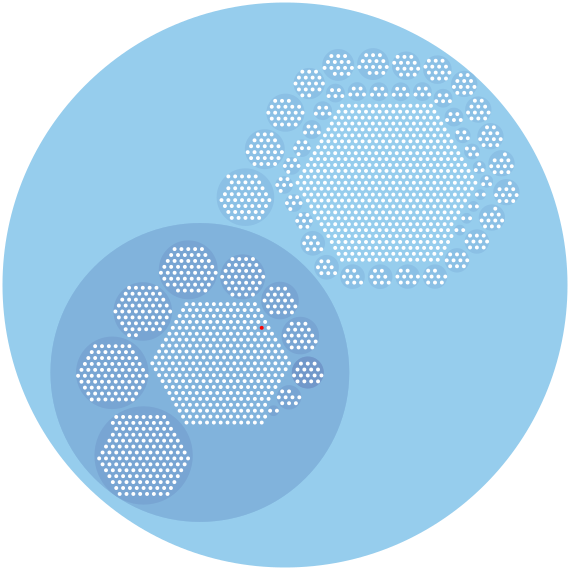
\includegraphics[width=0.47\textwidth]{figures/bubble_tree.pdf}
        \caption{Bubble Tree of merge 3f17ea6, merge 4dc4226 is the currently
          selected merge and is highlighted in orange.}
        \label{fig:bubble_tree}
\end{figure}

The bubble tree doesn't have an implicit way of providing additional
information, placing any text near the nodes makes the tree impossible
to read, so we include a separate pane in the web page. When a user
hovers over a node, the pane shows additional information about the
author and the commit message and a link to the detailed page for that
commit or merge. If the user clicks on a node, the tree will zoom to
that node and the information in the info pane will persist, enabling
the user to click the link. This tree provides an easy mechanism for
users to navigate from the root to the leaves and vice versa.

\section{Discussion}

From a developers point of view, the are two major disadvantages of the
DAG model of Git: a) its edges point backwards, i.e. commits point to
their ancestor, not to the commit that succeeds them on the path to
being integrated; and b) the DAG contains many more edges that are
necessary to understand how integration occurred. We addressed these two
issues with the creation of the merge-tree model from the DAG of Linux.
Effectively, the merge-tree recovers the details of how each
branch---and the commits they contain---was merged into the master
branch.

In our experience, no other Git repository reaches the level of DAG
complexity that Linux has. In most Git repositories, most merges are not
nested---most merges merge directly into the master repository, and
these merges only merge a few commits. Even in these simplified cases,
the merge-tree can provide a valuable summary of how commits are
integrated into the master branch, specifically since the time of
integration may be very different from the time the commits were
authored.

\evan{Check accuracy of this paragraph}

The biggest challenge is computing the merge-tree of any given
repository. It is likely that our heuristic for computing the merge-tree
will not work with other repositories. The heuristic requires that there
are no fast-forward merges into the master branch of the repository (a
majority of repositories), and that there are no foxtrot merges (a
practice that is starting to be considered desirable by git
users\footnote{See
  \url{http://devblog.nestoria.com/post/98892582763/maintaining-a-consistent-linear-history-for-git}
  and
  \url{https://developer.atlassian.com/blog/2016/04/stop-foxtrots-now/}}).
We are able to use our heuristic with the Linux kernel because of the
strict integration model imposed by Linus. To validate the results of
the heuristic, we use the continuous mining technique described in
\cite{German2015}.  Continuous mining of the repository requires
foresight and planning.

Because \tool leverages the merge-tree model of the kernel, it provides
mechanisms and visualizations that other tools are unable to produce. It
gives us the ability to see how commits are being merged into the master
branch, allowing us to better understand how code is integrated into the
kernel.

\begin{figure}
        \centering
        \includegraphics[width=0.47\textwidth]{figures/042dd_DAG.png}
        \caption{Merge Dag View}
        \label{fig:dag_view}
\end{figure}

\begin{figure}
        \centering
        \includegraphics[width=0.47\textwidth]{figures/042dd_tree.pdf}
        \caption{Merge tree topology for the same merge as in
                Figure~\ref{fig:dag_view}.}
        \label{fig:tree_view}
\end{figure}

Our goal was to build a tool to enable maintainers to effectively
navigate and browse the changes performed to the kernel over the period
of a release. Achieving this goal includes removing information that
does not pertain to the area of the kernel that the user is interested
in. In Figures~\ref{fig:dag_view} and \ref{fig:tree_view} we can
visually compare the results returned from Gitk and our tool for the
top-level merge ``042dd60ca6dec9a02cefa8edd67de386e35755d6'' from kernel
version 3.10. Note that Gitk has no way to show or recognize that this
is a merge into the master branch.

The log information to this merge-commit in both of these figures is
identical, but the presentation drastically changes our ability to
comprehend what we are seeing.  The primary difference is the removal of
irrelevant information. In Gitk (Figure~\ref{fig:dag_view}), the
visualization results include commits and merges from other components
of the kernel, while our tool (Figure~\ref{fig:tree_view}) only includes
the results that are specific to the component of the kernel that we are
interested in.

Even though this merge is relatively small, containing only four
sub-merges, three of which only contain a single commit, and the last
containing two commits, it is already hard to visualize in Gitk.  With
\tool we are able to immediately see what section of the kernel these
commits and merges pertain to. The DAG view of this provides almost no
explanation, furthermore, users must work to determine where this merge
ends and the next one begins.

\tool further enhances our understanding by summarizing the files and
modules that were edited in the entire branch being merged. We are able
to determine that three files, ``palamas-regulator.c'' had two lines
added and two lines removed, ``dbx500-prcmu.c'' had 12 lines added and
12 lines removed, and ``core.c'' had 5 lines added and 2 lines removed.
Finally, we are able to determine that only the ``regulator'' module was
modified in this merge and was modified by 5 commits.


\section{Related Works}
\label{sec:related_works}

% vim:set et sw=2 ts=4 tw=72:
% Jul 04, 2017
% Evan Wilde

\section{Related Works}
\label{sec:related_works}

Version control systems monitor the development lifetime of software
projects. This makes the version control system vital in providing
information about how a software project is being developed. To do this,
the user must be able to gain a clear understanding of how commits are
being integrated into the project, along with understanding what changes
these commits are bringing with them. These are the tasks that we set
out to solve with the \mt model. Ideally, we could compare our model
against another that is designed with these goals. To our knowledge, we
know of no git repository visualzation tool that has these specific
goals. This may be due to issues with finding the master branch of the
repository which is a non-trivial task, or due to other factors.

While we have found no tool with the express goal of showing how a
commit is integrated, and providing a summarization of a merge, there
has been a lot of work done in providing visualizations of various
aspects of a repository.

Many tools work to address the issues in communication between
developers in inter-team collaboration work. Codebook\cite{Begel2010}
uses a data mining technique to determine the developer of a piece of
code, the program manager who wrote the specification for the code, and
the program managers and developers on the team who were working
together. Hipikat\cite{Cubranic2005} is another tool with a focus on
communication. Where Codebook focuses on developers working on a
project, Hipikat is focused on enabling easier integration of new
developers to a project by providing them with easily-searchable
artifacts of the changes made. Codebook is useful for pairing a
contributor with the original developer; however, the developer may not
have worked with the piece of code in years. A Hipikat program may
provide more information to the maintainer as it records the artifacts
of why certain design decisions were made when they were made using
other tools like Bugzilla and CVS.\@ Neither tool is sufficient in
meeting our goals to provide a summary of the topology of the kernel
repository through a visual tree.

Most visualizers provide a visual presentation of a certain aspect of a
repository. Fractal Figures\cite{Ambros2005} uses a unit square to
represent a portion of a project, then partitions the square based on
the proportion of an author's contributions to that portion of the
project. EPOSee\cite{Burch2005} and Evolution Radar\cite{Ambros2009}
perform further analysis, determine which files are made together, and
what changes are made over a sequence of commits, though the goals
behind these projects is different.

Codebook, Hipikat, Fractal Figures, EPOSee, and Evolution Radar all work
with data from CVS repositories. Our goal is to provide information
about Git repositories, specifically the Linux master repository. Fewer
tools are available for generating visualizations and summaries of Git
repositories, potentially due to the DAG model used by Git.

Gource is a tool for providing an interactive timelapse of the state of
a repository\cite{Caudwell2010}. In the timelapse, it shows who
contributes and what type of contribution a developer is making. These
contribution types are one of, adding a file, removing a file, and
changing a file. While the timelapse is interesting to watch, it does
not provide any additional explanation of the changes actually being
made, only the frequency that they are being made and who is making
them.

% TODO: add code_swamp or something like that


% TODO: Check this -- Look into source tree
Git itself is shipped with summarization and visualization tools:
the \verb|git log| command and Gitk, which is a graphical tool for the purpose of browsing
the DAG of the repository.
Many other tools are designed with a similar visual metaphore
as what is presented in Gitk, including Git kraken, Github Desktop and
web interfaces, the Git Lab web intereface, the Bitbucket web interface,
and many others. The Gitk interface is built around the central DAG
viewer. The DAG displays the repository events on their respective
branches, the author, and the date that the event was authored. A user
can select an event to view addition information about it, including the
full commit log, the parents and children of the event, and the diff
generated if modifications were made. In the case of the Linux kernel,
merges are not resolved as merge conflicts in the master repository, but
by the developers prior to merging. With this development model, no
merges will have modified any files, and will not show a diff. While the
merge does not make changes directly, the effects of merging the
commits persist, but Gitk is unable to provide an aggregated view of the
files modified, the patches for those files, and the authors who
contributed commits to that merge.

Our tool is primarily aimed at presenting the hierarchical structure of
the Linux git repository. We use tables for presenting the summarized
information of the commits and merges, but this information could also
be presented in a graphical form. Various graphical forms for displaying
file and authorship data exist, the principal forms being matrix views,
city scapes, bar and pie charts, and networks \cite{Eick2002}. Any of
these data visualization metaphors are applicable to our system.

%%% Local Variables:
%%% mode: latex
%%% TeX-master: "lineval.tex"
%%% End:


\section{Controlled User Study}
\label{sec:study}

\dmg{start by describing what you mean by user study... to evaluate linvis we performed a user study...}

\dmg{and you are evaluating the visualizations, NOT the DAG}


We use a controlled mixed-methods users study in order to evaluate the
ability for the DAG to provide users with a conceptual image of how a
commit is integrated into a project, to compare the DAG and \mt models,
and determine which model the users preferred.

In this section, we describe the methods used to for designing and
implementing the user study.
\dmg{no, you describe the study, which includes the methods}

\dmg{Start by giving an overall overview of the study: the study consists of a set of tasks that users are expected to
  perform... do a top down description of what users will do
}

\subsection{Questions and Tasks}
\label{sub:questions}

\dmg{use tasks, not questions. you are asking them to do something that requires an answer, that is different than a question}


\begin{table*}[htpb]
  \centering
  \caption{Conceptual Tasks }
  \label{tab:conceptual_tasks}
  \begin{tabulary}{0.9\textwidth}{LL}
    \toprule
    Task & Description\\
    \midrule
    T1 & Draw a diagram showing how this commit was merged into the master branch, along with any other related commits\\
    T2 & How many individual commits are related to this commit?\\
    T3 & How many merges are involved with merging this commit into the master branch?\\
    \bottomrule
  \end{tabulary}
\end{table*}

\begin{table}[htpb]
  \centering
  \caption{Summarization Tasks}
  \label{tab:summarization_tasks}
  \begin{tabulary}{\linewidth}{LLL}
    \toprule
    Task Set   & Task & Description\\\midrule
    Merge      & T4   & What is the series of merges involved with merging this
    commit?\\
               & T5   & What other commits are merged?\\
    Authorship & T6   & How many authors are involved?\\
               & T7   & Who contributed the most changes?\\
    Files      & T8   & How many files were modified?\\
               & T9   & Which file had the most changes?\\
    Modules    & T10  & Which modules does this merge tree involve?\\
    \bottomrule
  \end{tabulary}
\end{table}

\dmg{avoid editorializing your text: remove purely}

\dmg{watch for tense... we don't begin... the tasks begin... or better, the first tasks...}

The questions and tasks are broken down into four groups. The first two
groups are purely quantitative in nature; the study begins with
conceptual tasks to understand whether the DAG is capable of providing
users with an understanding of how a commit is merged into the master
branch, and other commits that it is merged with. We continue with
summarization tasks, to quantitatively understand if the \mt model makes
a difference in summarization tasks.

The third task set is purely qualitative, \dmg{and are their goal is ... don't imply content in your sentences... be
  precise; this applies to the paragraph before} to gain better understanding
of whether participants preferred working with the \mt model in \tool,
or working with the DAG in Gitk, and what aspects they preferred from
each tool. The final group of questions is simply to gain a better
understanding of the demographic of our participants.


\textbf{Conceptual Tasks}


\dmg{given the choice, not allowed.  I don't understand this section.
  You need to be more top-down in your description. you need to provide
  context on what the users are expected to do, and why. So what are the
  tasks? You never explain.  what is the goal of the tasks? how many?
  what were the tasks? what is expected from each? you need to answer
  these questions, not necessarily in the same order.  also, remember
  this is a comparative study, so I presume the users were asked to do
  both with linvis and without it (choice of gitk/git command line) }

The participants were allowed to use Gitk or the git command line tools
to perform these tasks. These tasks are asked in the specified order,
allowing tabularr to first, create a conceptual understanding of the
commits and merges that will be involved with the rest of the tasks that
follow.tabularmay then use their diagrams to answer T2 and T3. We do not
collect metrics from \tool for the conceptual tasks, opting instead to
determine if the DAG is sufficient for understanding how a commit is
integrated. \tool uses the \mt model show a tree visualization of how
commits are merged, until the commit reaches the master branch.
Table~\ref{tab:conceptual_tasks} shows the conceptual tasks.

\dmg{I don't like the present tense, but that is your option}

We provide the participant with 10 minutes per commit to complete the
first task. The answers to the two other questions in this section are
drawn from the answer in the first task.

\textbf{Summarization Tasks}


\dmg{again, you are going into details first. First the tasks --see
  above-- including their grouping.  then at the end, describe the
  randomization and why it is done (which you did) }

The summarization tasks (Table~\ref{tab:summarization_tasks}) are
grouped into \dmg{how many?} set of tasks according to their theme. The
tasks within a given task set are shuffled, and the task sets are
shuffled, to ensure that similar questions are together, but not in the
same order, and to ensure that the themes are in randomized order
between participants. The order of the commits is shuffled, as well. The
order of the tool is randomized, choosing to start with either \tool or
Gitk, to ensure that we do not place a bias on one tool through the
experiment.

As understanding where the merge begins and ends is vital to answering
the other question, the merge task set will always be the first task set
presented; however, the questions will still be re-ordered within the
task set.

\textbf{User Opinion and Profile}

Finally, we ask the user for their opinions on the tools and for some
information about their level of experience with git.  \dmg{be more
  precise: understanding or preference is too broad. What you want to
  know answers to specific questions regarding how the tools compare and
  which ones they would prefer} The first three questions are intended
to provide us with a better understanding of preference, and insight on
why, the participant had that preference.  The last three questions in
this section are aimed at getting a better understanding of the
demographic of our participants.

\begin{enumerate}
  \item Given these tasks again, which tool would you prefer to use?
  \item Which aspects of each tool did you like and why?
  \item How long have you used git?
  \item If you have used git, for what kind of projects? (personal,
    school courses, professional?)
  \item If you have used git, how many commits, files, and contributors
    were involved with the largest repository you have worked with?
\end{enumerate}


\textbf{Procedure}

\dmg{tell me first why you need to create a script, so I know what you
  do something: we did random assignment of tasks (explain what you did)
  and randomized the order in which the tasks were performed.  Then
  explain why you need a script}

\dmg{it does not randomize the order the tools. It randomizes which tool
  is going to be used on each tasks.  be precise with your language}

\dmg{what you explained how commits relate to tasks and how they get
  assigned? think as if you are explaining this to somebody who has to
  do this: you are the designer, explaining the why and the how }

For each participant, we run a simple python script to generate the
script for the study, eliminating the possibility of bias from us. The
script randomizes the order of the tools, the order of the commits, the
order of the task sets, and the order of the tasks within each task set,
where appropriate.


\subsection{Commit Selection}
\label{sub:commit_selection}

\dmg{see my comments in previous section. it is ok to explain them here,
  but you need to explain what they are briefly in the previous section}

We chose two commits for use in the study. The order that the commits
are presented is randomized between participants, but the order is kept
consistent through the tasks described in the next subsection.

\dmg{this place does not require a description of the database. This
  requires just to say the commits/merge set (dates and numbers are ok)
  only} We use the \tool database, containing commits and merge-tree
information from April 16th 2005 to October 14th, 2014, which
corresponds to being between Linux release 2.6.12-rc3 and Linux
3.17-rc1. \evan{Cite the database even more?} \dmg{again, i have
  problems with your writing: ``we wanted to use in the study commits of
  different size, to determine if the size had an impact in the
  completion of the tasks. We chose commits of three different sizes...}
We chose the commits based on tree sizes. We \dmg{we didn't find: this
  is a fact, not a discovery; what is a majority? 50\%+1? be precise}
\dmg{drop the word inner, and do it in order: 25\% of trees have only
  one commit, 50\%.., 75\%...} found that a majority of the trees
contain at most seven inner commits, while more than 25\% of the trees
contain a single commit. 75\% of the tree contained up to 51 inner
commits and merges, and finally the largest tree contained 7217 nodes.
We chose to work with the trees in \dmg{if you are going to use the
  words quartile, just use them before in your description eg: the
  distribution of the sizes of the trees is x, y merges, whose size
  corresponded to the 25 ,50 quartiles, simple and precisee} the first
and second quartile, as merge trees of sizes between one and seven, not
including the merge into the master branch, make up the majority of the
trees in the database.

\dmg{remove from here, what is here? this is not a road trip :)} From
here, we selected one tree from the trees of a single commit at random.
Selecting a commit from that tree is trivial, as there is only one to
choose.\dmg{remove the obvious, instead concentrate on why the others
  are not trivial}

We selected one tree of size seven at random from all trees of size
seven\dmg{how many where there?}. We placed a restriction the trees, the
selected tree must include at least one internal merge to increase the
complexity of the trees tested. For each randomly selecting a tree, we
chose one of its internal commits at random (using the
\verb|random.choice| function in python 3.6.1).

\dmg{question: so you chose only one commit of each size, and the
  randomization was which tool to use for each question? or did they
  have to do the same task for two commits?}

Using this technique, we selected commit
\emph{a3c1239eb59c0a907f8be5587d42e950f44543f8} from the tree containing
a single node (Figure~\ref{fig:commit_1}), which we will refer to as
\comA, and commit \emph{cdbdd1676a5379f1d5cbd4d476f5e349f445befe}, from
the tree containing seven nodes (Figure~\ref{fig:commit_2}), which we
will refer to as \comB.

\begin{figure}[bpt]
  \centering
\begin{tabular}{ m{1.5cm} m{3cm} }
  \includegraphics[height=0.5in]{figures/commits/1-commit.pdf} &
  \includegraphics[height=1in]{figures/commits/7-commits.pdf}\\
\end{tabular}
  \caption{The merge trees used in the user study, 
    containing one and seven commits, respectively.}
  \label{fig:commit_1}
\end{figure}


\subsection{Results}
\label{sec:results}

\dmg{this is still methodology.}

We recorded the audio and screen capture video for each participant in
the study for further analysis.
\dmg{you don't need this sentence, it is redundant}
After capturing the information, we
extracted various metrics from the videos.
\dmg{ you don't record, you measure}
From the conceptual tasks, we
recorded the time in seconds, and the answer for the question. We
extracted three metrics for the summarization tasks, the time in
seconds, the correctness, and the accuracy.
\dmg{and then somethings you are over precise :): correctness is simply whether their answer to the task was correct or not}
Correctness is a binary
value, it is true if the response was correct and false if the response
was incorrect.
\dmg{if you are going to use this metric, you need to define precisely. remember, you are giving this to somebody else
  to implement}
The accuracy is measures in distance from the correct
value. An accuracy of zero indicates a correct answer. All tasks in the
summarization tasks include an accuracy metric except T7, which will
only be right or wrong, and therefore cannot meaningfully be measured by
a distance.

\subsection{Conceptual Tasks}
\label{sub:conceptual_tasks}

\dmg{i don't like the expression: we are able to see... too long.. be to the point: Table X shows/depicts/ etc ... they
  are not overviews, they are a summary}
In Table~\ref{tab:conceptual_results}, we are able to see an overview of
the results from the conceptual questions.


\begin{table*}[htpb]
  \centering
  \caption{Results from the conceptual questions\dmg{what are the columns? they need captions}}
  \label{tab:conceptual_results}
  \begin{tabular}{ll|r|lrr|rrr}
    Question                      & Commit & Answer & Median & Mean  & Variance & Median(s) & Mean(s) & Variance(s)\\\hline\hline
    Number of commits in the tree & \comA  & 1      & 4      & 19.11 & 753.11   & 10.0      & 49.92   & 5952.08\\
    Number of merges in the tree  & \comA  & 1      & 5      & 8.27  & 53.62    & 7.5       & 24.67   & 884.42\\\hline
    Number of commits in the tree & \comB  & 5      & 4      & 7.80  & 136.84   & 31.5      & 106.83  & 54123.42\\
    Number of merges in the tree  & \comB  & 3      & 3.5    & 5.40  & 50.27    & 11.0      & 65.6    & 29798.82\\
  \end{tabular}
\end{table*}

Users were able to more closely estimate the number of commits and
merges in the larger tree, but generally took longer than the smaller
tree. The tree with a single node resulted in more variability in the
estimate of number of commits.

It should be noted that these questions were answered after spending
roughly ten minutes attesting to draw a picture that held the answers to
these questions.

\subsection{Summarization Tasks}
\label{sub:summarization_tasks}

In Figure~\ref{fig:summarization_results}, we see all of the
correctness, accuracy, and timing results. The first row of plots are
the correctness results. We see in all cases except for T10, that the
number of instances of a correct result with \tool is roughly the same
as the number of incorrect instances with Gitk. We test each task with
the McNemar Chi-square test~\cite{McNemar1947}.

\begin{figure*}[htpb]
  \centering
  \includegraphics[width=\textwidth]{figures/userstudy/results.pdf}
  \caption{Results from the summarization tasks. The first row plots the
    correctness metric for each task. The second row plots the
    accuracy metric for each task. The third row plots the time metric
    for each task.}
  \label{fig:summarization_results}
\end{figure*}

With the McNemar's tests, we analyze the participants that change from
being correct with one tool to being incorrect with the other. This does
not take into account the number of people who were able to provide the
correct answer for both tools, nor the people who were incorrect for both
tools. The results show whether providing the participants with \tool
over the current standard, gitk, improves the correctness of the
summarization tasks among the participants. We show the results for the
number of people who were, with both tools, correct, incorrect, and
changed in Table~\ref{tab:correctness_table}.

In all cases, except for task T10, we saw statistically significant
results suggesting that we reject the null hypothesis. We tested each
correctness with an $\alpha = 0.005$. The $\chi^2$ test value with one
degree of freedom is $7.879$.

\begin{table*}[htpb]
  \centering
  \caption{Correctness tables showing how many people stayed correct,
    incorrect, and how many people changed between tool}
  \label{tab:correctness_table}
  \begin{tabular}{c|c|c}

    T4 & T5 & T6\\
  \begin{tabular}{cc|rr}
                           &           & \multicolumn{2}{c}{Linvis}\\
                           &           & Correct                      & Incorrect\\\hline
    \multirow{2}{*}{Gitk}  & Correct   & 6                            & 0\\
                           & Incorrect & 15                           & 2\\
  \end{tabular} &

  \begin{tabular}{cc|rr}
                           &           & \multicolumn{2}{c}{Linvis}\\
                           &           & Correct                      & Incorrect\\\hline
    \multirow{2}{*}{Gitk}  & Correct   & 5                            & 0\\
                           & Incorrect & 14                           & 4\\
  \end{tabular}

  &

  \begin{tabular}{cc|rr}
                           &           & \multicolumn{2}{c}{Linvis}\\
                           &           & Correct                      & Incorrect\\\hline
    \multirow{2}{*}{Gitk}  & Correct   & 5                            & 0\\
                           & Incorrect & 16                           & 2\\
  \end{tabular}


  \\\hline
  T7 & T8 & T9\\

  \begin{tabular}{cc|rr}
                           &           & \multicolumn{2}{c}{Linvis}\\
                           &           & Correct                      & Incorrect\\\hline
    \multirow{2}{*}{Gitk}  & Correct   & 8                            & 0\\
                           & Incorrect & 13                           & 2\\
  \end{tabular}  &
  \begin{tabular}{cc|rr}
                           &           & \multicolumn{2}{c}{Linvis}\\
                           &           & Correct                      & Incorrect\\\hline
    \multirow{2}{*}{Gitk}  & Correct   & 6                            & 0\\
                           & Incorrect & 15                           & 2\\
  \end{tabular} &
  \begin{tabular}{cc|rr}
                           &           & \multicolumn{2}{c}{Linvis}\\
                           &           & Correct                      & Incorrect\\\hline
    \multirow{2}{*}{Gitk}  & Correct   & 6                            & 0\\
                           & Incorrect & 14                           & 3\\
  \end{tabular}\\\hline

  & T10 & \\
  & \begin{tabular}{cc|rr}
                            &           & \multicolumn{2}{c}{Linvis}\\
                            &           & Correct                      & Incorrect\\\hline
    \multirow{2}{*}{Gitk}   & Correct   & 14                           & 1\\
                            & Incorrect & 8                            & 0\\
  \end{tabular} & \\

  \end{tabular}
\end{table*}

The correctness test statistics and conclusion for each summarization
task;

The correctness test statistics, conclusions, and a description of the
accuracy and timing results for each summarization task follow:

\begin{itemize}

  \item

    T4; the resulting $\chi^2$ value is $15$. $15 > 7.879$, therefore we
    reject the null hypothesis that \tool does not make a difference in
    the correctness when determining the series of merges that a commit
    takes, with $99.5\%$ confidence.

    There is almost no variation in accuracy between participants using
    \tool, while there is more variance in Gitk. There were two outliers
    among the instances using \tool, which lie within the second and
    third quartiles for the accuracy measure of Gitk. The furthest
    outlier for \tool lies at a distance that is slightly greater than
    the median for Gitk.

    We see similar results in the timing metric; all significant data
    occurs within less time than the second, third, and fourth quartile
    of the Gitk results. Nearly all outlier instances in \tool are
    within the third quartile group of the instances of Gitk with the
    exception of the most extreme, which lies in the fourth quartile
    group.

    The results indicate that \tool is able to assist users with
    determining how a commit is merged more accurately, and more
    quickly.

  \item

    T5; the resulting $\chi^2$ value is $14$. $14 > 7.879$, therefore we
    reject the null hypothesis that \tool does not make a difference in
    the correctness when determining the other related commits, with
    $99.5\%$ confidence.

    There is very little variance in the accuracy of results for \tool
    compared to the accuracy of the results in Gitk. The median distance
    is smaller, indicating that the participants performed more
    accurately using \tool.

    There is less variance in the time taken to come to an answer with
    \tool than with Gitk. Furthermore, we see that a majority of the
    participants were able to complete the task in \tool in much less
    time than 50\% of the participants using Gitk.

    The results indicate that \tool is able to assist users in
    understanding which commits are related to a given commit.

  \item

    T6; the resulting $\chi^2$ value is $16$. $16 > 7.879$, therefore we
    reject the null hypothesis that \tool does not make a difference in
    the correctness when determining the number of authors involved with
    the merge tree, with $99.5\%$ confidence.

    We see the same results from this task as with the previous tasks,
    suggesting that \tool assists users determine the number of authors
    more quickly and more accurately.

  \item

    T7; the resulting $\chi^2$ value is $13$. $13 > 7.879$, therefore we
    reject the null hypothesis that \tool does not make a difference in
    the correctness when determining who contributed the most changes,
    with $99.5\%$ confidence.

    This question does not include an accuracy metric, as there are only
    two possible outcomes. We see the same result in the timing metric
    as we did from the previous questions.

    The results suggest that \tool is able to help users correctly
    identify the person who contributed the most lines of code to a
    merge tree in less time.

  \item

    T8; the resulting $\chi^2$ value is $15$. $15 > 7.879$, therefore we
    reject the null hypothesis that \tool does not make a difference in
    the correctness when determining how many files were contributed,
    with $99.5\%$ confidence.

    The results of this task are the same as in the previous tasks.
    This suggest that \tool is able to assist users determine how many
    files were modified, more quickly and more accurately.

  \item

    T9; the resulting $\chi^2$ value is $14$. $14 > 7.879$, therefore we
    reject the null hypothesis that \tool does not make a difference in
    the correctness when determining which file had the most changes,
    with $99.5\%$ confidence.

    While this question appears to have a similar answer to the correct
    answer for T7, the answer \comA had two files with the same number
    of midifications, thus the participant must correctly identify both
    of these files to be correct. For this reason, we include an
    accuracy metric.

    The results of this task are the same as the previous tasks.
    This suggests that \tool is able to assist users to determine which
    file had the most changes.

  \item

    T10; the resulting $\chi^2$ value is $5.44$. $5.44 < 7.879$,
    therefore we do not reject the null hypothesis, suggesting that
    \tool does not make a difference in determining which modules are
    involved with a merge tree.

    The accuracy and timing results for this task are the same as the
    others, showing that there is less variability in both accuracy and
    the time taken to have an answer between participants using \tool
    than using Gitk. Looking Table~\ref{tab:correctness_table}, we can
    see that, unlike the other questions, a majority of the participants
    were correct using both tools.

\end{itemize}

\subsection{User Opinions}
\label{sub:user_opinions}

Among the 12 pariticipants, there was nearly unanimous agreement that
for conceptual understanding and summarization tasks, \tool was easier
to work with than Gitk. The participants cited the ability to abstract
information about the merge from the clean summarization tables and
simple visualizations. Three participants suggested that someone with a
professional understanding of Gitk and the git commandline may be to
extract the a good conceptual understanding from the DAG, and perform
the summarization tasks from the commandline. One of these three
participants said that they would prefer to have both tools available,
as they are able to complement eachother.

\section{Discussion}
\label{sec:discussion}

% TODO: Go back to the conceptual task results and make them stronger
Overall, the results show fairly conclusive results; the DAG is unable
to adequately provide users with an explanation of the changes being
made in the repository, the DAG is not easily understood, and the DAG is
unable to provide summarizations of the changes being made at a merge.
Meanwhile, the \mt model is able to provide a better explanation of how
a commit is integrated, along with better summarization capabilities. In
this section, we discuss some observations made during the study,
threats to the validity of the study, comments made by the participants
during the study, modifications to the original algorithm to help
generalize it for more repositories, and future work.

\subsection{Observations}
\label{sub:observations}

% TODO: include info on merge tree sizes

During the course of the study, we noticed a consistent theme among the
participants. The most difficult challenge was identifying the master
branch of the repository. Given that single-commit merge trees are the
most common tree, and that they are relatively simple, we were
interested in seeing if the participants would be able to identify the
tree easily, but the results suggest that this was not the case. The
issue primarily stemmed from not being able to identify the master
branch. Most of the participants realized that they should not be going
backward, toward the initial commit, very early on. Furthermore, many
would identify the correct commit; however, they would start listing
every merge along the master branch as being a merge in the tree, and
including the commits from that merge. In the case of the single commit,
simply identifying the master branch would most likely be sufficient in
providing a clearer understanding of how a commit or flat tree is
integrated into the master branch of the repository.

While, in general, the participants of the study preferred using \tool
to Gitk, there were some noticeable usability issues. The most prominent
issue being the navigation within the tree. The participants expected
that the tabs would update when they clicked on a node in the tree,
instead of having to click the link to the commit after clicking the
node. This was true in both the Reingold-Tilford tree and the Pack tree.
The second major usability issue was the inconsistency between the list
tree and the other tree visualizations. The list tree is rooted at the
repository event that the user is current looking at, while the other
tree visualizations show the entire tree, and use bright orange to
highlight the current node.


\subsection{Comments From a Release Manager}
\label{sub:comments_from_a_release_manager}

One of the participants of the study had worked as a release manager for
more than three years, working with both SVN and CVS repositories, but
had little experience with git.

Contributors making merges need to understand more than just what merges
a commit was collected into before reaching the repository of the
contributor. It is also important to understand order that the related
commits were made, as they tell the story of what the developer was
thinking as they were writing the changes. The current merge-tree model
does not order the commits, simply placing them randomly. This is the
primary reason behind this participant's request to use both
simultaneously. \tool is able to help with the aggregation of the
information, and provide a better understanding of the next merge
involved in integrating this commit, but the DAG in gitk provides the
full story of the commit instead of hiding it behind a layer of
abstraction.

The comments from this participant were very insightful, and will assist
in improving the model in the future.

\subsection{Threats to Validity}
\label{sub:threats}

While git includes gitk and the git log provides a view of the DAG with
\verb|git log --graph|, many of the participants in our study were
unfamiliar with the DAG visualizations shown by these tools. A possible
reason for this may be that unless a repository reaches a sufficient
complexity, both in branching and number of commits, these tools are
necessary for the normal operation of git. Furthermore, fear of the
complexity caused by branching may cause personal and academic
repositories to have relatively simple structures. While they were
unfamiliar with the DAG structure, these users were also unfamiliar with
the \mt model, and were still able to better understand and summarize
the repository using \tool.

Each question was evaluated independently of the results from the
previous question in the summarization tasks. Had we modified the
correct answer to fit the conceptual understanding of which commits were
included in the tree, we may have witnessed different results. A
modification to the study may include providing the participants with
the correct set of commits prior to the summarization tasks, after the
merge task set.


\subsection{Generalization}
\label{sub:generalization}

Seeing that the \mt model is able to assist users with understanding how
commits are integrated, we continue by looking at ways of improving the
algorithm for faster operations, and making the conversion from DAG to
\mt feasible over the internet for smaller repositories.

The problem of finding the master branch is the most difficult, and is
not possible without heuristic approaches. The master branch can be
confounded by \textit{foxtrot} merges, which change the order of the
parents in the parent list of a merge. Other than the ordering of the
parent list, git has no other way to determine which commits are on the
master branch of the repository. For the purpose of this discussion, we
will assume that we can rely on the order of the parent list to be
correct, and that foxtrots do not occur.

\begin{algorithm}
  \caption{Computing the generalized Merge Tree}
  \label{alg:generalized}
  \begin{algorithmic}[1]
    \Function{Phase 1}{initial commit $root$} : updated tree
    \State $depth \gets 0$
    \State $Q \gets root$
    \Do
    \State $cur \gets Q.dequeue$
    \State $parents \gets cur.parents$
    \State $depth \gets depth + parents.length - 1$
    \For{$index, parent \in parents$}
    \If{$parent.depth$ is $undefined$}
    \State $parent.depth \gets cur.depth + index$
    \ElsIf {$cur.depth > parent.depth$}
    \State $depth \gets depth - 1$
    \ElsIf {$cur.depth < parent.depth$}
    \State $depth \gets depth - 1$
    \State $parent.depth \gets cur.depth$
    \EndIf
    \State $parent.children \gets cur$
    \If{$parent$ has not been visited}
    \State $Q \gets parent$
    \State $parent.visited \gets True$
    \EndIf
    \EndFor
    \doWhile{$Q$ not empty and $depth \ne 0$ }
    \EndFunction

    \Function{Phase 2}{initial commit $root$} : Merge tree
    \State $tree.root \gets root$
    \State $Q$ // Empty Queue

    \State $parents \gets root.parents$
    \State $parents \gets tail\ parents$
    \For {$parent \in parents$}
    \State $realParent \gets min(\forall child \in parent.children,\ parent.depth >= child.depth)$
    \If {$realParent$ is $root$}
    \State $root.children \gets parent$
    \State $parent.parent \gets root$
    \State $Q \gets parent$
    \EndIf
    \EndFor

    \While{$Q$ not empty}
    \State $cur \gets Q.dequeue$
    \State $parents \gets cur.parents$
    \For{$parent \in parents$}
    \State $realParent \gets min(\forall child \in parent.children,\ parent.depth >= child.depth)$
    \If {$realParent$ is $cur$}
    \State $cur.children \gets parent$
    \State $parent.parent \gets cur$
    \State $Q \gets parent$
    \EndIf

    \EndFor
    \EndWhile

    \EndFunction
  \end{algorithmic}
\end{algorithm}

The primary difference between the original algorithm and the
generalization is the main data structure. Algorithm~\ref{alg:original}
is centered around the use of the stack, making it akin to a depth-first
traversal of the DAG.\@ The generalization in
Algorithm~\ref{alg:generalized} is based on the queue, making it akin to
the breadth-first traversal of the DAG.\@ While the final results of the
two traversals should not be different, the runtime properties are
different.

We will begin with a simplified description of the original algorithm.
We start at the master branch pointer. We will use the term master
branch loosely here, meaning any branch that has been labeled in some
way as being the main branch, this branch may have a different name, but
standard naming conventions call it the master branch. Starting from the
master branch label, we traverse the entire master branch to the initial
commit, recording the commit hash of every repository event encountered.

The second phase iterates over every commit, computing the shortest
distance to the master branch. For this reason, the entire repository
must be available to the algorithm. This is a dynamic programming
solution, centered around the call stack. The next node on the shortest
path to the master branch will become the parent of this node in the
tree.

If this algorithm is to be generalized into a dynamic, web-based, tool,
it may not be feasible to download every commit in the repository in a
reasonable period of time. We instead look toward a breadth-first
approach at limiting the number of repository events that must be
downloaded.

Focusing on the generalized algorithm~\ref{alg:generalized}, the
algorithm is broken into two phases. The first phase is where the
improvements take place. The first phase has three main goals, the first
is to track the master branch. The second goal labels the depth of each
repository event that is traverses. The final goal is to record the
children of each commit, reversing the DAG.\@ The first phase also
begins the process of reversing the DAG, by providing the candidate
commits that could possibly be the real parent to this node. The first
phase can terminate early, if it reaches a point where all branches that
it is following terminate. The depth metric on line 7 indicates how many
branches are currently being traversed. In line 11 through 15, we
decrement the depth, as this is the point where a branch occurs. The
changing of the depth occurs if there are more events on the same branch
than between the merge and branch point of a separate branch.

\begin{table}[htpb]
  \centering
  \caption{Example traversal of the example DAG in
    Figure~\ref{fig:repoDAG} starting at merge 11.}
  \label{tab:ex_traversal}
  \begin{tabular}{cccc|cc}
    \toprule
    Current & Parents & Depth & Q       & Visited & Children\\\midrule
    -       & -       & 0     & 11      & 11:0    & \\
    11      & 4,9     & 1     & 4,9     & 4:0     & 11, 5\\
    4       & 1       & 1     & 9,1     & 9:1     & 11\\
    9       & 7,6,8   & 3     & 1,7,6,8 & 7:1     & 9, 8\\
    1       &         & 3     & 7,6,8   & 6:2     & 9\\
    7       & 5       & 3     & 6,8,5   & 8:3     & 9\\
    6       & 5       & 2     & 8,5     & 5:1     & 7, 6\\
    8       & 7       & 1     & 5       & 2:1     & 5, 3\\
    5       & 4,2,3   & 2     & 2,3     & 3:2     & 5\\
    2       & 1       & 1     & 3       &         & \\
    3       & 2       & 0     &         &         & \\
    \bottomrule
  \end{tabular}
\end{table}

In Table~\ref{tab:ex_traversal}, we follow the algorithm starting at
merge commit 11 from the example in Figure~\ref{fig:repoDAG}, recording
the current node, the parents of the current node, the depth after
updating, and the queue structure after updating. The visited column is
not dependant on the current step, but keeps track of the nodes that
have been visited, and the depth at that node. When we reverse the DAG,
the children in this table will become the candidates for being the
parent of the corresponding node. For example, the parent of node 7 may
be resolved to either node 9 or node 8. In this case, the shortest path
to the master branch is through node 9.

The terminology surrounding the parent/child relationship gets very
confusing at the change between phase one and two because this is where
the roles switch. In phase 1, we are working with the DAG; in phase 2,
we are working with a structure that is neither a tree nor a DAG, but
can only be described as a directed graph.

The goal of the second phase is to resolve the tree from the directed
graph. We will refer to parents in the same sense as we would refer to
them in the tree form of the repository for the remainder of this
section. We have gathered the depths and possible parents (line 17), but
we need to remove the extra parents. Extra parents are culled in line
42 of the algorithm. Of the possible parents, we take the parent that is
closest to the root, but not beyond. This forces the real parent to
either be deeper in the tree, or on the same branch. Line 30 to 37 are
for bootstrapping the queue, ensuring that we are not starting on an
empty queue.

The construction of the tree becomes trivial now that we are able to
determine the parents and children for each node. Lines 44 and 45
perform this construction, adding the DAG parent to the tree children of the
current node, and the DAG parent's parent becomes the current node,
which was the DAG parent's child. We continue following the path until
we hit the root node, merging the commit into the master branch.

This algorithm relies heavily on the order of parents in the parent
list, but is able to trim the number of nodes that must be downloaded.
Furthermore, the resulting tree is able to show the order of commits,
telling the story of how a developer was working, before the set of
commits was merged. We developed a small bitbucket plugin to test the
design and determine whether it was capable of producing merge trees,
shown in Figure~\ref{fig:b_plugin}.

\begin{figure}[htpb]
  \centering
  \includegraphics[width=\linewidth]{figures/plugin.png}
  \caption{Screen shot of the Bitbucket plugin showing the online tree
    computation of the repository shown in~\ref{fig:repoDAG}.}
  \label{fig:b_plugin}
\end{figure}

\section{Conclusion}
\label{sec:conclusion}

In this paper, we develop a tree-based model designed to provide git
users with a better explanation of the events occurring in a git
repository. The \mt model is rooted at the merge into the master branch
of a repository, where the leaves are the individual commits.

We implement a tool, \tool, which allows a user to filter the commits
with a simple search interface. Once the user finds the commit that they
are interested in, they are provided simple aggregated tables showing
the files that were modified, the authors that made the modifications,
among other information. They are also provided with three
visualizations, a list tree, a pack tree, and a Reingold-Tilford tree
view. The list tree enables easy searching for textual features, while
the pack tree is good for visualizing the structure of large merge
trees, and the Reingold-Tilford tree is better at visualizing the
structure of small merge trees.

To ensure that our model is necessary, we evaluate the ability of users
to perform simple conceptual tasks, finding how a commit was merged into
the master branch of the Linux repository, and determining other commits
that were merged with the given merge. Finding that the participants in
our study were unable to perform this task, we compared the ability of
the participants to summarize key pieces of information aggregated in
these groups of commits. We asked for information about what files were
modified, the authors making the changes, among other tasks. Finally, we
asked the participants about their preference in tools, and which
aspects of each they preferred. We found that the participants in our
study were able to correctly identify the correct answer more quickly
using the \mt model than they were able to with the DAG.

Given that the model provides users with a better understanding of
events in the repository, we describe some issues with identifying the
master branch of the repository and a more generalized approach to
constructing merge trees. We implement the generalized approach as a
bitbucket plugin to verify that it is able to quickly produce results
online, unlike in the implementation of \tool.



% TODO: You can tell that I am tired. This conclusion will need to be re-worked.

\balance

% \nocite{*}

\bibliographystyle{IEEEtran}
\bibliography{references}

\end{document}

%%% Local Variables:
%%% mode: latex
%%% TeX-master: t
%%% End:
